

%% bare_conf.tex
%% V1.4b
%% 2015/08/26
%% by Michael Shell
%% See:
%% http://www.michaelshell.org/
%% for current contact information.
%%
%% This is a skeleton file demonstrating the use of IEEEtran.cls
%% (requires IEEEtran.cls version 1.8b or later) with an IEEE
%% conference paper.
%%
%% Support sites:
%% http://www.michaelshell.org/tex/ieeetran/
%% http://www.ctan.org/pkg/ieeetran
%% and
%% http://www.ieee.org/

%%*************************************************************************
%% Legal Notice:
%% This code is offered as-is without any warranty either expressed or
%% implied; without even the implied warranty of MERCHANTABILITY or
%% FITNESS FOR A PARTICULAR PURPOSE! 
%% User assumes all risk.
%% In no event shall the IEEE or any contributor to this code be liable for
%% any damages or losses, including, but not limited to, incidental,
%% consequential, or any other damages, resulting from the use or misuse
%% of any information contained here.
%%
%% All comments are the opinions of their respective authors and are not
%% necessarily endorsed by the IEEE.
%%
%% This work is distributed under the LaTeX Project Public License (LPPL)
%% ( http://www.latex-project.org/ ) version 1.3, and may be freely used,
%% distributed and modified. A copy of the LPPL, version 1.3, is included
%% in the base LaTeX documentation of all distributions of LaTeX released
%% 2003/12/01 or later.
%% Retain all contribution notices and credits.
%% ** Modified files should be clearly indicated as such, including  **
%% ** renaming them and changing author support contact information. **
%%*************************************************************************


% *** Authors should verify (and, if needed, correct) their LaTeX system  ***
% *** with the testflow diagnostic prior to trusting their LaTeX platform ***
% *** with production work. The IEEE's font choices and paper sizes can   ***
% *** trigger bugs that do not appear when using other class files.       ***                          ***
% The testflow support page is at:
% http://www.michaelshell.org/tex/testflow/



\documentclass[conference]{IEEEtran}
% Some Computer Society conferences also require the compsoc mode option,
% but others use the standard conference format.
%
% If IEEEtran.cls has not been installed into the LaTeX system files,
% manually specify the path to it like:
% \documentclass[conference]{../sty/IEEEtran}





% Some very useful LaTeX packages include:
% (uncomment the ones you want to load)


% *** MISC UTILITY PACKAGES ***
%
%\usepackage{ifpdf}
% Heiko Oberdiek's ifpdf.sty is very useful if you need conditional
% compilation based on whether the output is pdf or dvi.
% usage:
% \ifpdf
%   % pdf code
% \else
%   % dvi code
% \fi
% The latest version of ifpdf.sty can be obtained from:
% http://www.ctan.org/pkg/ifpdf
% Also, note that IEEEtran.cls V1.7 and later provides a builtin
% \ifCLASSINFOpdf conditional that works the same way.
% When switching from latex to pdflatex and vice-versa, the compiler may
% have to be run twice to clear warning/error messages.






% *** CITATION PACKAGES ***
%
%\usepackage{cite}
% cite.sty was written by Donald Arseneau
% V1.6 and later of IEEEtran pre-defines the format of the cite.sty package
% \cite{} output to follow that of the IEEE. Loading the cite package will
% result in citation numbers being automatically sorted and properly
% "compressed/ranged". e.g., [1], [9], [2], [7], [5], [6] without using
% cite.sty will become [1], [2], [5]--[7], [9] using cite.sty. cite.sty's
% \cite will automatically add leading space, if needed. Use cite.sty's
% noadjust option (cite.sty V3.8 and later) if you want to turn this off
% such as if a citation ever needs to be enclosed in parenthesis.
% cite.sty is already installed on most LaTeX systems. Be sure and use
% version 5.0 (2009-03-20) and later if using hyperref.sty.
% The latest version can be obtained at:
% http://www.ctan.org/pkg/cite
% The documentation is contained in the cite.sty file itself.






% *** GRAPHICS RELATED PACKAGES ***
%
\ifCLASSINFOpdf
  % \usepackage[pdftex]{graphicx}
  % declare the path(s) where your graphic files are
  % \graphicspath{{../pdf/}{../jpeg/}}
  % and their extensions so you won't have to specify these with
  % every instance of \includegraphics
  % \DeclareGraphicsExtensions{.pdf,.jpeg,.png}
\else
  % or other class option (dvipsone, dvipdf, if not using dvips). graphicx
  % will default to the driver specified in the system graphics.cfg if no
  % driver is specified.
  % \usepackage[dvips]{graphicx}
  % declare the path(s) where your graphic files are
  % \graphicspath{{../eps/}}
  % and their extensions so you won't have to specify these with
  % every instance of \includegraphics
  % \DeclareGraphicsExtensions{.eps}
\fi
% graphicx was written by David Carlisle and Sebastian Rahtz. It is
% required if you want graphics, photos, etc. graphicx.sty is already
% installed on most LaTeX systems. The latest version and documentation
% can be obtained at: 
% http://www.ctan.org/pkg/graphicx
% Another good source of documentation is "Using Imported Graphics in
% LaTeX2e" by Keith Reckdahl which can be found at:
% http://www.ctan.org/pkg/epslatex
%
% latex, and pdflatex in dvi mode, support graphics in encapsulated
% postscript (.eps) format. pdflatex in pdf mode supports graphics
% in .pdf, .jpeg, .png and .mps (metapost) formats. Users should ensure
% that all non-photo figures use a vector format (.eps, .pdf, .mps) and
% not a bitmapped formats (.jpeg, .png). The IEEE frowns on bitmapped formats
% which can result in "jaggedy"/blurry rendering of lines and letters as
% well as large increases in file sizes.
%
% You can find documentation about the pdfTeX application at:
% http://www.tug.org/applications/pdftex





% *** MATH PACKAGES ***
%
%\usepackage{amsmath}
% A popular package from the American Mathematical Society that provides
% many useful and powerful commands for dealing with mathematics.
%
% Note that the amsmath package sets \interdisplaylinepenalty to 10000
% thus preventing page breaks from occurring within multiline equations. Use:
%\interdisplaylinepenalty=2500
% after loading amsmath to restore such page breaks as IEEEtran.cls normally
% does. amsmath.sty is already installed on most LaTeX systems. The latest
% version and documentation can be obtained at:
% http://www.ctan.org/pkg/amsmath





% *** SPECIALIZED LIST PACKAGES ***
%
%\usepackage{algorithmic}
% algorithmic.sty was written by Peter Williams and Rogerio Brito.
% This package provides an algorithmic environment fo describing algorithms.
% You can use the algorithmic environment in-text or within a figure
% environment to provide for a floating algorithm. Do NOT use the algorithm
% floating environment provided by algorithm.sty (by the same authors) or
% algorithm2e.sty (by Christophe Fiorio) as the IEEE does not use dedicated
% algorithm float types and packages that provide these will not provide
% correct IEEE style captions. The latest version and documentation of
% algorithmic.sty can be obtained at:
% http://www.ctan.org/pkg/algorithms
% Also of interest may be the (relatively newer and more customizable)
% algorithmicx.sty package by Szasz Janos:
% http://www.ctan.org/pkg/algorithmicx




% *** ALIGNMENT PACKAGES ***
%
%\usepackage{array}
% Frank Mittelbach's and David Carlisle's array.sty patches and improves
% the standard LaTeX2e array and tabular environments to provide better
% appearance and additional user controls. As the default LaTeX2e table
% generation code is lacking to the point of almost being broken with
% respect to the quality of the end results, all users are strongly
% advised to use an enhanced (at the very least that provided by array.sty)
% set of table tools. array.sty is already installed on most systems. The
% latest version and documentation can be obtained at:
% http://www.ctan.org/pkg/array


% IEEEtran contains the IEEEeqnarray family of commands that can be used to
% generate multiline equations as well as matrices, tables, etc., of high
% quality.




% *** SUBFIGURE PACKAGES ***
%\ifCLASSOPTIONcompsoc
%  \usepackage[caption=false,font=normalsize,labelfont=sf,textfont=sf]{subfig}
%\else
%  \usepackage[caption=false,font=footnotesize]{subfig}
%\fi
% subfig.sty, written by Steven Douglas Cochran, is the modern replacement
% for subfigure.sty, the latter of which is no longer maintained and is
% incompatible with some LaTeX packages including fixltx2e. However,
% subfig.sty requires and automatically loads Axel Sommerfeldt's caption.sty
% which will override IEEEtran.cls' handling of captions and this will result
% in non-IEEE style figure/table captions. To prevent this problem, be sure
% and invoke subfig.sty's "caption=false" package option (available since
% subfig.sty version 1.3, 2005/06/28) as this is will preserve IEEEtran.cls
% handling of captions.
% Note that the Computer Society format requires a larger sans serif font
% than the serif footnote size font used in traditional IEEE formatting
% and thus the need to invoke different subfig.sty package options depending
% on whether compsoc mode has been enabled.
%
% The latest version and documentation of subfig.sty can be obtained at:
% http://www.ctan.org/pkg/subfig




% *** FLOAT PACKAGES ***
%
%\usepackage{fixltx2e}
% fixltx2e, the successor to the earlier fix2col.sty, was written by
% Frank Mittelbach and David Carlisle. This package corrects a few problems
% in the LaTeX2e kernel, the most notable of which is that in current
% LaTeX2e releases, the ordering of single and double column floats is not
% guaranteed to be preserved. Thus, an unpatched LaTeX2e can allow a
% single column figure to be placed prior to an earlier double column
% figure.
% Be aware that LaTeX2e kernels dated 2015 and later have fixltx2e.sty's
% corrections already built into the system in which case a warning will
% be issued if an attempt is made to load fixltx2e.sty as it is no longer
% needed.
% The latest version and documentation can be found at:
% http://www.ctan.org/pkg/fixltx2e


%\usepackage{stfloats}
% stfloats.sty was written by Sigitas Tolusis. This package gives LaTeX2e
% the ability to do double column floats at the bottom of the page as well
% as the top. (e.g., "\begin{figure*}[!b]" is not normally possible in
% LaTeX2e). It also provides a command:
%\fnbelowfloat
% to enable the placement of footnotes below bottom floats (the standard
% LaTeX2e kernel puts them above bottom floats). This is an invasive package
% which rewrites many portions of the LaTeX2e float routines. It may not work
% with other packages that modify the LaTeX2e float routines. The latest
% version and documentation can be obtained at:
% http://www.ctan.org/pkg/stfloats
% Do not use the stfloats baselinefloat ability as the IEEE does not allow
% \baselineskip to stretch. Authors submitting work to the IEEE should note
% that the IEEE rarely uses double column equations and that authors should try
% to avoid such use. Do not be tempted to use the cuted.sty or midfloat.sty
% packages (also by Sigitas Tolusis) as the IEEE does not format its papers in
% such ways.
% Do not attempt to use stfloats with fixltx2e as they are incompatible.
% Instead, use Morten Hogholm'a dblfloatfix which combines the features
% of both fixltx2e and stfloats:
%
% \usepackage{dblfloatfix}
% The latest version can be found at:
% http://www.ctan.org/pkg/dblfloatfix




% *** PDF, URL AND HYPERLINK PACKAGES ***
%
%\usepackage{url}
% url.sty was written by Donald Arseneau. It provides better support for
% handling and breaking URLs. url.sty is already installed on most LaTeX
% systems. The latest version and documentation can be obtained at:
% http://www.ctan.org/pkg/url
% Basically, \url{my_url_here}.




% *** Do not adjust lengths that control margins, column widths, etc. ***
% *** Do not use packages that alter fonts (such as pslatex).         ***
% There should be no need to do such things with IEEEtran.cls V1.6 and later.
% (Unless specifically asked to do so by the journal or conference you plan
% to submit to, of course. )
\usepackage{float}
\usepackage[]{placeins}
\usepackage{wrapfig}
\usepackage{graphicx}
\usepackage{fixltx2e}
\usepackage{caption}
\usepackage{subcaption}
\usepackage{dblfloatfix}
\graphicspath{ {images/} }
% correct bad hyphenation here
\hyphenation{op-tical net-works semi-conduc-tor}

\setlength{\parskip}{1em}
\renewcommand{\baselinestretch}{1.0}

\newcommand*{\addheight}[2][.5ex]{%
	\raisebox{0pt}[\dimexpr\height+(#1)\relax]{#2}%
}
\begin{document}
%
% paper title
% Titles are generally capitalized except for words such as a, an, and, as,
% at, but, by, for, in, nor, of, on, or, the, to and up, which are usually
% not capitalized unless they are the first or last word of the title.
% Linebreaks \\ can be used within to get better formatting as desired.
% Do not put math or special symbols in the title.
\title{Upper-body detection using R-CNN}


% author names and affiliations
% use a multiple column layout for up to three different
% affiliations
\author{\IEEEauthorblockN{Nguyen Phan Manh Hung}
\IEEEauthorblockA{Honours Program\\
Faculty of Information Technology\\
University of Science, VNU-HCM\\
Email: nguyenphanmanhhung@gmail.com}
\and
\IEEEauthorblockN{Nguyen Hoang Khanh Duy}
\IEEEauthorblockA{Honours Program\\
Faculty of Information Technology\\
University of Science, VNU-HCM\\
Email: nguyenhoangkhanhduy@gmail.com}
\and
\IEEEauthorblockN{Luc Kien Nghiep}
\IEEEauthorblockA{Honours Program\\
Faculty of Information Technology\\
University of Science, VNU-HCM\\
Email: luckiennghiep@gmail.com}}

% conference papers do not typically use \thanks and this command
% is locked out in conference mode. If really needed, such as for
% the acknowledgment of grants, issue a \IEEEoverridecommandlockouts
% after \documentclass

% for over three affiliations, or if they all won't fit within the width
% of the page, use this alternative format:
% 
%\author{\IEEEauthorblockN{Michael Shell\IEEEauthorrefmark{1},
%Homer Simpson\IEEEauthorrefmark{2},
%James Kirk\IEEEauthorrefmark{3}, 
%Montgomery Scott\IEEEauthorrefmark{3} and
%Eldon Tyrell\IEEEauthorrefmark{4}}
%\IEEEauthorblockA{\IEEEauthorrefmark{1}School of Electrical and Computer Engineering\\
%Georgia Institute of Technology,
%Atlanta, Georgia 30332--0250\\ Email: see http://www.michaelshell.org/contact.html}
%\IEEEauthorblockA{\IEEEauthorrefmark{2}Twentieth Century Fox, Springfield, USA\\
%Email: homer@thesimpsons.com}
%\IEEEauthorblockA{\IEEEauthorrefmark{3}Starfleet Academy, San Francisco, California 96678-2391\\
%Telephone: (800) 555--1212, Fax: (888) 555--1212}
%\IEEEauthorblockA{\IEEEauthorrefmark{4}Tyrell Inc., 123 Replicant Street, Los Angeles, California 90210--4321}}




% use for special paper notices
%\IEEEspecialpapernotice{(Invited Paper)}




% make the title area
\maketitle

% As a general rule, do not put math, special symbols or citations
% in the abstract
\begin{abstract}
Human dectection is an important technique used in many other problems such as traffic control, movies' features extracting, etc. However, it's hard to detect the whole body because the lower part is usually obscured by other objects like bikes, cars, tables, etc. This motivates us to use R-CNN to detect upper-body of the target. The experimental result using this technique achieves the accuracy of 95.5 \%. The dataset consists of 300 images. People in these images are from different ages and have different angles. This method can be improved by using better dataset.
\end{abstract}

% no keywords




% For peer review papers, you can put extra information on the cover
% page as needed:
% \ifCLASSOPTIONpeerreview
% \begin{center} \bfseries EDICS Category: 3-BBND \end{center}
% \fi
%
% For peerreview papers, this IEEEtran command inserts a page break and
% creates the second title. It will be ignored for other modes.
\IEEEpeerreviewmaketitle



\section{Introduction}
% no \IEEEPARstart
The increasing development of machine learning provide us more tools for different kind of detection problems. One of the problems is human detection in images. Human detection is an important step to solves other important problems such as the pedestrian detection system in self-driving cars or surveillance camera systems. However, human bodies are mostly obscured by other objects like bikes, cars, tables, trees, etc. This is an obstacle that can dramatically decrease the accuracy of full-body detection algorithms. That's why the authors recommend detecting upper body only using Region-based Convolutional Neural Networks.

There are many methods used for human detection, including SVM with discrete Wavelet transform \cite{wavelet} and HOG\cite{hog}. However, these methods have some disadvantages. For example, if images have low contrast and unclear boundaries due to some factors such as light or low-quality cameras, the images will provide incomplete gradient information, the fact that dramatically decreases the accuracy of detectors. To get rid of these disadvantages, we can apply some image preprocessing techniques. However, each image has different characteristics, therefore requires different techniques to preserve its properties. 
%This prevents systems from detecting humans from images extracted from videos due to 

The core idea of our method is using R-CNN trained with the dataset of humans' upper-body. To improve the accuracy, we pre-train the model using a large auxiliary dataset, ILSVRC, as recommended by \cite{rcnn}. After trained with 300 images, the origin model achieves the accuracy of 90\% [need to fix]. The modified model give a better result with the accuracy of 95.5\% [need to fix].

The rest of this paper is organized as follows. In section II, the authors describe dataset and methodology use to train and validate the model. In section III, we discuss about our model used in this paper. Section IV presents the experimental results and evaluations. The conclusions and future work are presented in section V. 

% An example of a floating figure using the graphicx package.
% Note that \label must occur AFTER (or within) \caption.
% For figures, \caption should occur after the \includegraphics.
% Note that IEEEtran v1.7 and later has special internal code that
% is designed to preserve the operation of \label within \caption
% even when the captionsoff option is in effect. However, because
% of issues like this, it may be the safest practice to put all your
% \label just after \caption rather than within \caption{}.
%
% Reminder: the "draftcls" or "draftclsnofoot", not "draft", class
% option should be used if it is desired that the figures are to be
% displayed while in draft mode.
%
%\begin{figure}[!t]
%\centering
%\includegraphics[width=2.5in]{myfigure}
% where an .eps filename suffix will be assumed under latex, 
% and a .pdf suffix will be assumed for pdflatex; or what has been declared
% via \DeclareGraphicsExtensions.
%\caption{Simulation results for the network.}
%\label{fig_sim}
%\end{figure}

% Note that the IEEE typically puts floats only at the top, even when this
% results in a large percentage of a column being occupied by floats.


% An example of a double column floating figure using two subfigures.
% (The subfig.sty package must be loaded for this to work.)
% The subfigure \label commands are set within each subfloat command,
% and the \label for the overall figure must come after \caption.
% \hfil is used as a separator to get equal spacing.
% Watch out that the combined width of all the subfigures on a 
% line do not exceed the text width or a line break will occur.
%
%\begin{figure*}[!t]
%\centering
%\subfloat[Case I]{\includegraphics[width=2.5in]{box}%
%\label{fig_first_case}}
%\hfil
%\subfloat[Case II]{\includegraphics[width=2.5in]{box}%
%\label{fig_second_case}}
%\caption{Simulation results for the network.}
%\label{fig_sim}
%\end{figure*}
%
% Note that often IEEE papers with subfigures do not employ subfigure
% captions (using the optional argument to \subfloat[]), but instead will
% reference/describe all of them (a), (b), etc., within the main caption.
% Be aware that for subfig.sty to generate the (a), (b), etc., subfigure
% labels, the optional argument to \subfloat must be present. If a
% subcaption is not desired, just leave its contents blank,
% e.g., \subfloat[].


% An example of a floating table. Note that, for IEEE style tables, the
% \caption command should come BEFORE the table and, given that table
% captions serve much like titles, are usually capitalized except for words
% such as a, an, and, as, at, but, by, for, in, nor, of, on, or, the, to
% and up, which are usually not capitalized unless they are the first or
% last word of the caption. Table text will default to \footnotesize as
% the IEEE normally uses this smaller font for tables.
% The \label must come after \caption as always.
%
%\begin{table}[!t]
%% increase table row spacing, adjust to taste
%\renewcommand{\arraystretch}{1.3}
% if using array.sty, it might be a good idea to tweak the value of
% \extrarowheight as needed to properly center the text within the cells
%\caption{An Example of a Table}
%\label{table_example}
%\centering
%% Some packages, such as MDW tools, offer better commands for making tables
%% than the plain LaTeX2e tabular which is used here.
%\begin{tabular}{|c||c|}
%\hline
%One & Two\\
%\hline
%Three & Four\\
%\hline
%\end{tabular}
%\end{table}


% Note that the IEEE does not put floats in the very first column
% - or typically anywhere on the first page for that matter. Also,
% in-text middle ("here") positioning is typically not used, but it
% is allowed and encouraged for Computer Society conferences (but
% not Computer Society journals). Most IEEE journals/conferences use
% top floats exclusively. 
% Note that, LaTeX2e, unlike IEEE journals/conferences, places
% footnotes above bottom floats. This can be corrected via the
% \fnbelowfloat command of the stfloats package.

\section{Background and Related Work}
Given a set of objects, the main goal of detection problem is to localize these objects in images, videos, or pieces of musics. This problem is difficult than the classification problem, in which we have to build a model that, given a object, can map it into a particular set specified by the problem. Formally, given $x \in D^n$ and a discrete set $R = \{y_0, y_1, ... y_m\}$, we have to build a transformation $F: D^n \rightarrow R$ that satisfies some constraints. However, there are many paradigms allowing us to utilize well known classifiers as detectors in our problems.

These paradigms usually have 2 main stages, whose structure will be discussed in the next section. 
\subsection{The objects proposal stage}
The main goal of this stage is to propose a set of image's portions that is likely to contain the target objects. For this reason, it's important to choose an appropriate algorithm to produce a good set of candidate objects because no matter how well the classifier performs, if the number of candidates is insufficient or the objects extracted from the images are badly affected, the overall accuracy of the detector system will drastically decrease. Fortunately, there are many methods, divided into 2 types which base on grouping super-pixels and sliding windows \cite{slidingwin5}, both simple and complex to solve the problem.
\begin{itemize}
	\item \textbf{Sliding Window.} \cite{slidingwin1}\cite{slidingwin2} We use rectangles of different sizes sliding over images. The set of images' portions, called sub-images, covered by those rectangles will be used as inputs for the classifier next stage. 
	
	For better results, before fed to the classifier, those sub-images should be evaluated by some function $F_{score}$ and then removed if their scores are below a specific threshold. In this way, we can speed up the whole system. For example, we want to detect people in images. Suppose that we have a sub-image where there isn't any change of image's brightness or color, which shows that the sub-image contains purely background information. Instead of feeding it to the classifier, which eventually classify it as the background, we can get rid of it from the beginning, using simple evaluation. 
	
	Additionally, sizes of windows, or the ratio between edges in particular, should be chosen carefully. To be clear, let examine a human's face detector. It's likely that humans' faces fit into squares or rectangles with approximately equal sides. Therefore, if we choose a window with ratio between sides approximate 5:1, the classifier may fail to recognize the face.
	
	Another way to use this technique in detection problem is to decompose the interest object into many parts \cite{slidingwin4}. Each part is then detected by a specific type of window and combined to get the original object.
	
	In conclusion, this technique is simple and efficient but has high computational complexity in practice due to the redundancy of sub-images.  
	\item \textbf{Local interest point} \cite{localinterestpoint1} Instead of considering all the windows, we only need to concern the areas around interested points extracted from images. In this way, we can decrease the number of candidate object dramatically.
\end{itemize} 
%This stage plays an important role in detection problems because regions suggested will be used as candidate objects for the classifier next stage. Therefore,  
\subsection{The classifier stage}

After being proposed by the previous stage, in this stage, proposed regions are examined more carefully using other algorithms.
To classify these object, we don't usually use the pixels directly. The two popular methods are appearance-based method and feature-based method. 
Appearance based method uses example images to perform this stage, but changes in lighting or color, changes in view direction, and changes in size or shape can fail our system. Edge matching, greysacle matching and gradient matching are some of appearance-based methods.

The other method is feature-based method. In this method, we usually extract some features from objects to use instead of using the pixels directly.\cite{realtimeface}. The reason they explained in \cite{realtimeface} is because feature an act to encode ad-hoc domain knowledge that is difficult to learn using a finite quantity of data and the feature based system operates much faster than a pixel based system. There are a lot of feature we can use. 

In face detection\cite{realtimeface}, Paul and Michael use Rectangle feature. \\
\begin{figure}
	\centering
	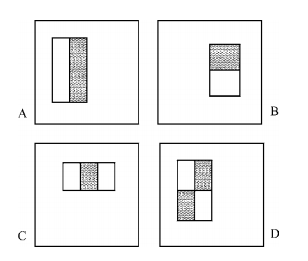
\includegraphics[width = 0.5\textwidth]{rectangleFeature}
	\caption{Example rectangle features shown relative to the enclosing detection window. The sum of the pixels which lie within the white rectangles are ubtracted from the sum of pixels in the grey rectangles \cite{realtimeface}}
\end{figure}
Them sum of pixels which lie within the white rectangles are substracted from the sum of pixels in the grey rectangles. Using intergral image \cite{realtimeface}, we can compute any rectangle feature rapidly. Other popular feature we can use are SIFT, SURF, HOG, etc.
\section{Method}
Our system is divided into following part:
\begin{enumerate}
	\item Object localization
	\item Pre-training
	\item Supervised fine-tuning
\end{enumerate}	

\subsection{Region proposal network}
%There're many ways, which are mentioned above, to localize objects in images such as sliding window, local interest point, etc. 
In this paper, we use Region Proposal Network (RPN)\cite{slidingwin5} to suggest regions for the classifier. RPN takes images of multiple sizes as input and outputs pairs of 
(proposed   region\footnote{"proposed region" is an abstract term. The shape of a proposed region depends on algorithms, objects, problems, etc. However, in this problem, we use rectangle regions because it's simple and efficient enough to solve the problem.}, objectness score\footnote{The objectness score measures the probability if the proposed region is a object or not.}).
\subsubsection{Generate Region}
We treat the feature maps generated by the last shared convolutional layer \footnote{The RPN and the classifier share a convolutional feature maps to reduce the computational cost.} as input images and slide the RPN over the feature maps. Each sliding window is then mapped into a lower dimensional feature and fed into 2 fully connected layers, called box regression layer and box classification layer correspondingly. The box regression layer predicts coordinates of the bounding box associated to each anchor. The box classification layer computes the corresponding objectness score of each proposed region.

Each sliding window is associated to an abstract object called anchor. The anchor is placed at the center of the sliding window and includes scale and aspect ratio of the proposal region. By using anchors, we can predict regions of any shape without changing scale and aspect ratio of the sliding window. 

This approach, using shared RPN and the sliding window, has 2 important properties.

\begin{enumerate}
	\item \emph{Translation invariance} By using the shared RPN and the sliding window, the detector can tolerate the translation of objects. Furthermore, using shared RPN allows reducing size of the model, therefore requires fewer traning data to achieve an equivalent accuracy.  
	\item \emph{Multi-scale object} There are many ways to deal with multi-scale objects such as image-pyramid in HOG and multi-scale sliding windows. The former is efficient but time-consuming. The latter is also efficient and sometimes is used together with the first one. In this paper, we use multi-scale anchors instead, which allows us to use fixed-size images/feature maps and sliding windows. This is more efficient than methods mentioned above in term of time complexity.
\end{enumerate}

\subsubsection{Training}
To train RPN, we use stochastic gradient descent and back-propagation. The loss function is:
\begin{equation}\label{eq:RPN_loss}
L(p, l, \hat{p}_g, \hat{l}_g) = \frac{1}{N_{cls}}L_{cls}(l^i, \hat{l}^i_g) + \frac{1}{N_{reg}} L_{reg}(p^i, \hat{p}^i_g)
\end{equation}
In \ref{eq:RPN_loss}, $$p^i$$ is vector representing the coordinate of the bounding box predicted by regression layer associated with anchor $$i$$ of mini-batch samples and $$l^i$$ is the probability that region $$i$$ contains object or not. Similarly, $$p^i_g$$ is the coordinate of the ground-truth bounding box, and $$l^i_g$$ is the ground-truth label of region $$i$$.

Finally, to train RPN, we use back-propagation and stochastic gradient descent through 100000 iterations. Learning rate, weight decay, and momentum is 0.001, 0.0005, and 0.9 correspondingly.
\subsection{Pre-training}
Due to the enormous number of parameters, the model we use, Zeiler and Fergus model, requires a huge amount of training examples, which takes much time a to collect and label. To address the issue, we first initialize the model by training it with images from ILSVRC 2012 and then fine-tune the domain of our model by Uper-Body dataset. In this way, the model can learn a higher level of abstract features before trying to learn from the specific dataset of the problem. %adding more comparison between 2 model - pre-train & not pre-train
\subsection{Supervised fine-tuning}
Many algorithms are proposed to address human detection problem. Most of them achieve high accuracy when whole body is captured or only obscured a little. We use upper-body dataset for training model, concerning the fact that humans in "wild environment" are usually obscured by other object such as tables, cars, motorbikes, etc. To be clear, take a look at \ref{fig:h_exp1}. In this image, the lower parts of these people are hidden by the car. Therefore, should any detectors try find humans in this image by searching whole bodies, they will fail.
\begin{figure}
	\centering
	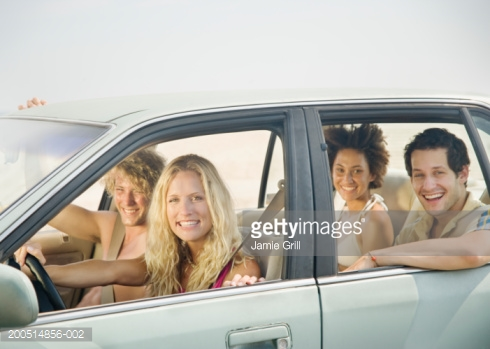
\includegraphics[width = 0.4\textwidth]{img7}
	\caption{}
	\label{fig:h_exp1}
\end{figure}

We divide the dataset into 4 classes: face wide \footnote{front face}, face side, upper body wide \footnote{the part above belly}, upper body side. Dividing upper-body dataset into 4 sub-classes allows the model to learn common features of each class better than to learn features of a super class, upper-body, only. Additionally, by using symmetric transformation, model can learn both left/right side of face/upper-body simultaneously.
\section{Experiment results}
The authors retrain the model with a different dataset to solve the Upper Body Detection problem. The dataset contains 98 images of people or groups of people. The authors concern 4 types of upper body, which is used as 4 classes for the ground truth.\\
The 4 types of upper body are: face\_wide, face\_side, upper\_body\_wide (ub\_wide), upper\_body\_side (ub\_side)
The number of images that each class appears in is as the table below:

\begin{center}
	\begin{tabular}{|c|c|c|c|}
		\hline
		\textbf{face\_wide} & \textbf{face\_side} & \textbf{upper\_body\_wide} & \textbf{upper\_body\_side}\\ 
		\hline
		51 & 43 & 31 & 62 \\
		\hline
	\end{tabular}
\end{center}

To rate the result, we recommend a new scale:\\
Let R = \((C - W) / A\)

Where:\\
R (rating) is the rating of the detection algorithm on a specific test. We want to maximize this value. And we can use this value to tell if one algorithm is better than another.\\
C (correct) is the number of correct objects (upper body or face) detected.\\
W (wrong) is the number of objects that is mistakenly detected.\\
A (all) is the total number of faces and upper bodies appeared in the images used for testing.\\

Let see why this formula works. We want to maximize C to reach A (the total number of objects in the test). Thus, \(C / A\) is pretty much the right formula for this detection problem. It represents the posibility that an object will be detected. The higher this value is, the better our algorithm is. But we don't want to forget that sometimes our detection system fails to detect an object and claims one object to be another. So we add the W value to the formula. In that way even the algorithm manages to detect all the objects in the test, but meanwhile mistake other objects to be faces or upper bodies, it still gets a bad rating. 

The authors run the model on 5 tests. Each test contains 10 images. After that, we calculate the R values for each test and calculate the average value avg(R).

The results can be desmonstrated by the following images:
%\begin{figure}
%	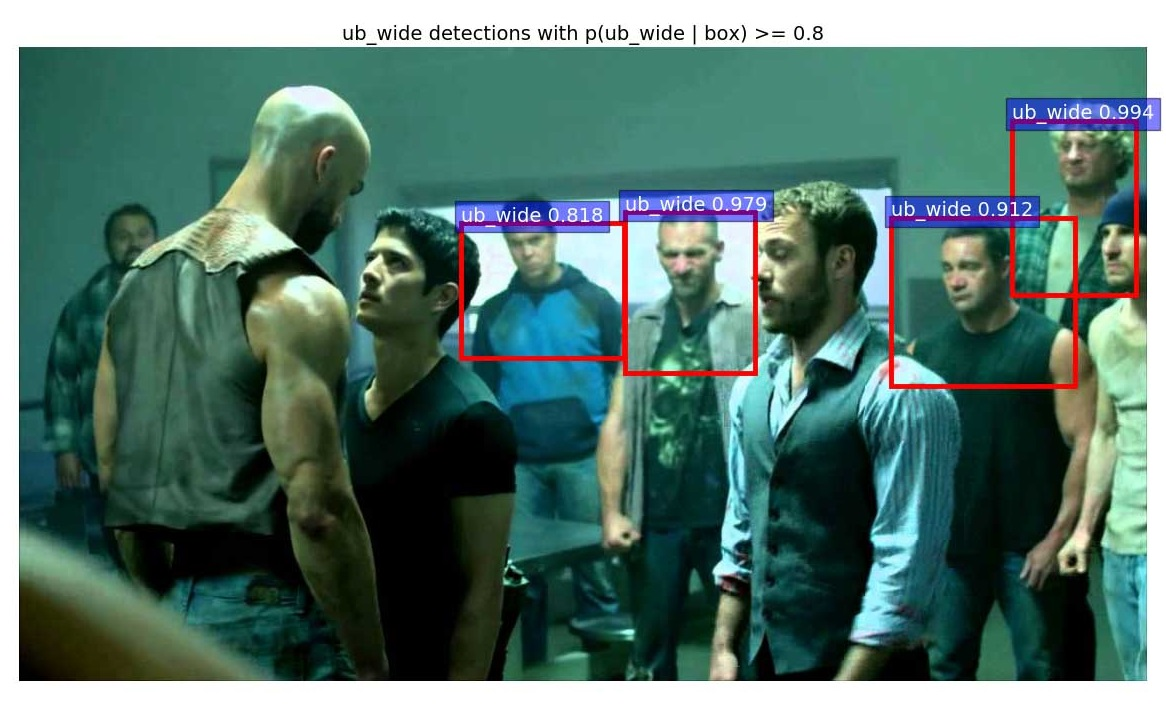
\includegraphics[width=0.7\linewidth]{img1}
%	\caption{}
%	\label{fig:res1}
%\end{figure}
\begin{figure*}[h]
	\centering
	\begin{subfigure}[b]{0.3\textwidth}
		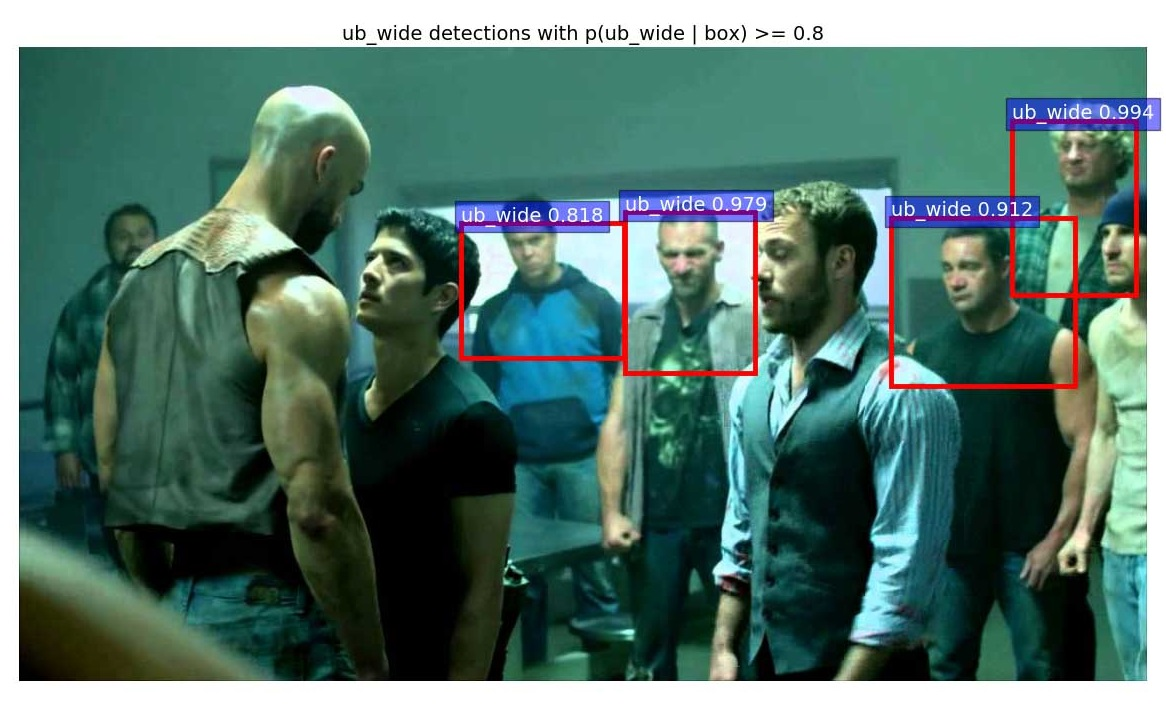
\includegraphics[width=\textwidth]{img1}
		\caption{}
		\label{fig:res1}
	\end{subfigure}
	~
	\begin{subfigure}[b]{0.3\textwidth}
		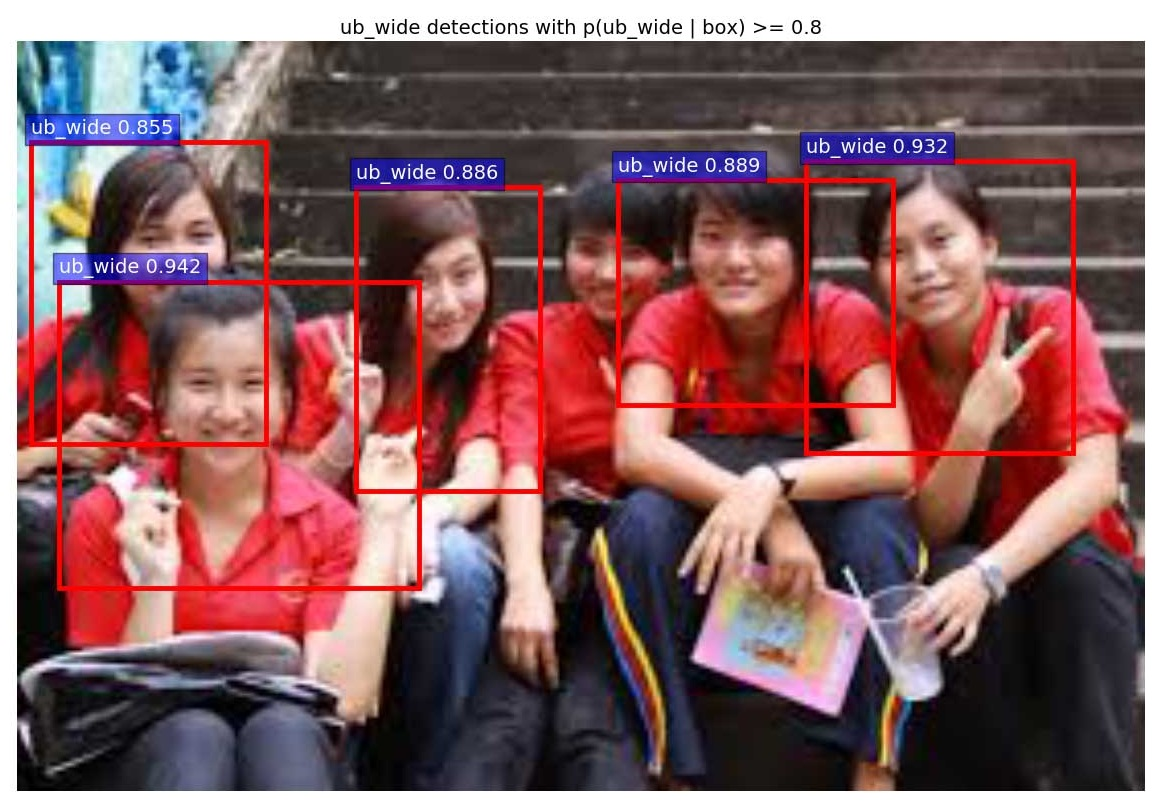
\includegraphics[width=\textwidth]{img2}
		\caption{}
		\label{fig:res2}
	\end{subfigure}
	~ %add desired spacing between images, e. g. ~, \quad, \qquad, \hfill etc. 
	%(or a blank line to force the subfigure onto a new line)
	\begin{subfigure}[b]{0.3\textwidth}
		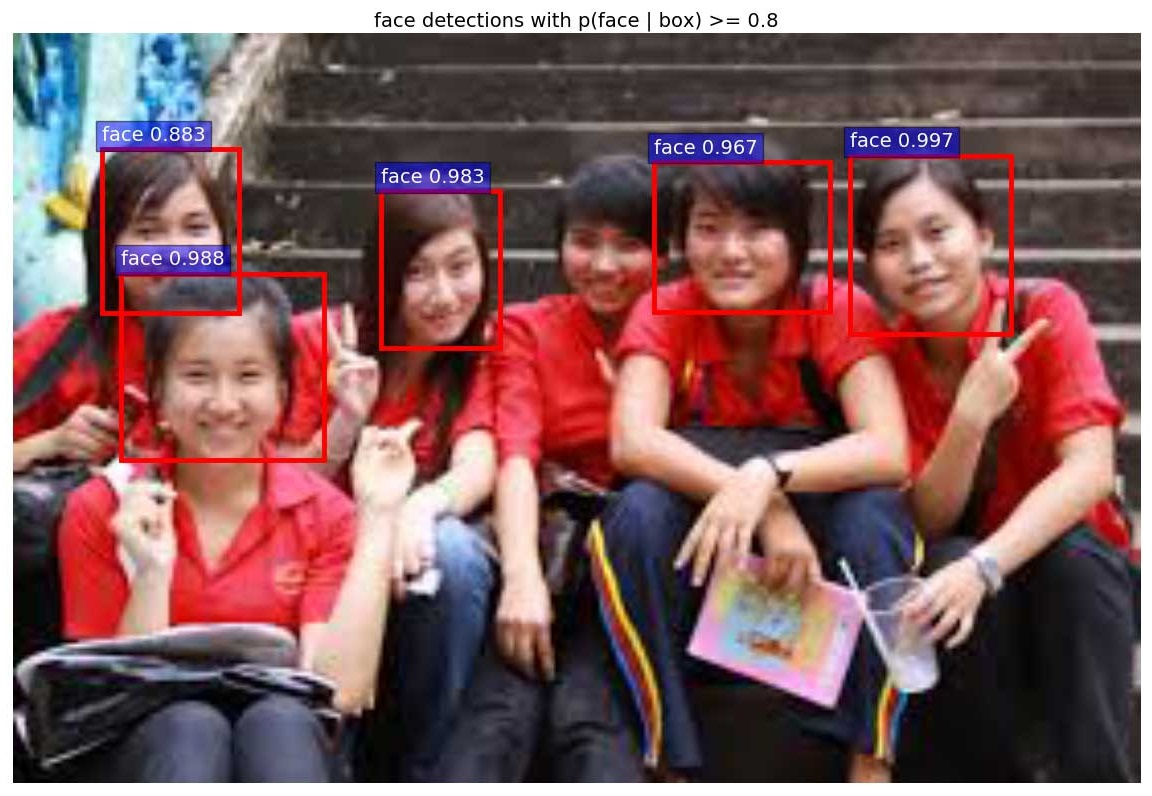
\includegraphics[width=\textwidth]{img3}
		\caption{}
		\label{fig:res3}
	\end{subfigure}
	~ %add desired spacing between images, e. g. ~, \quad, \qquad, \hfill etc. 
	%(or a blank line to force the subfigure onto a new line)
	\begin{subfigure}[b]{0.3\textwidth}
		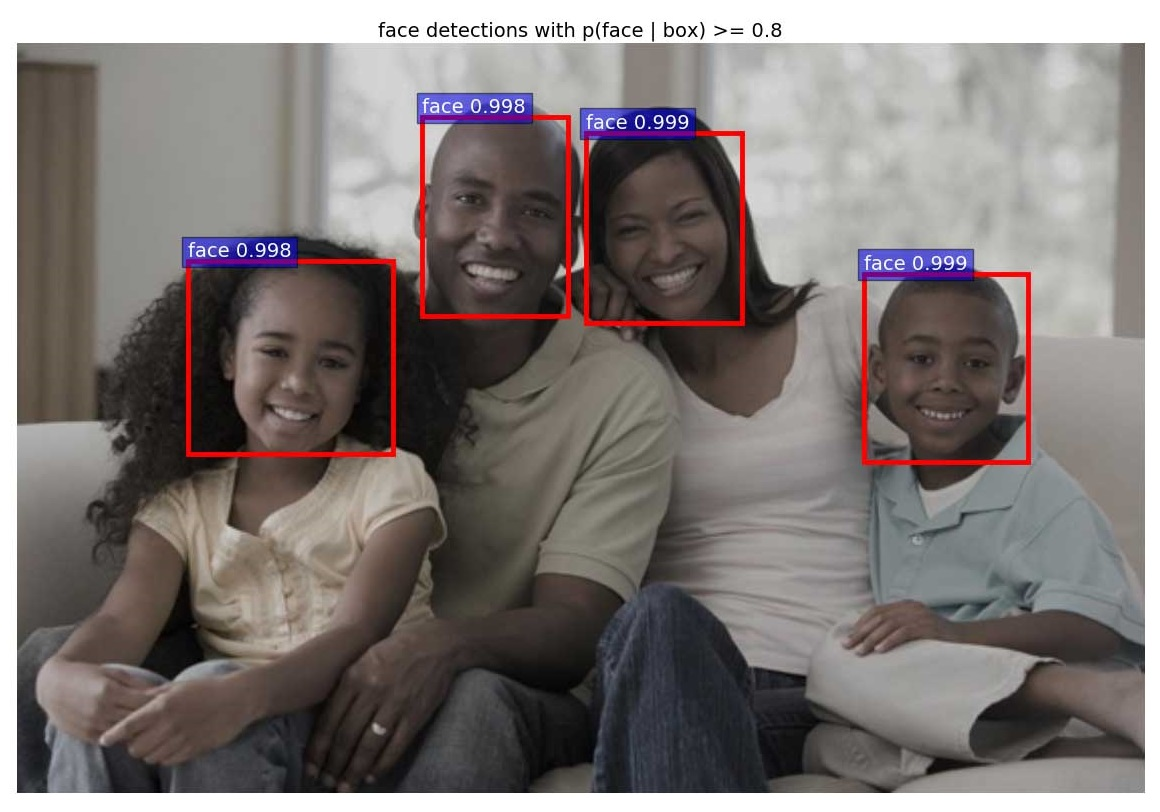
\includegraphics[width=\textwidth]{img4}
		\caption{}
		\label{fig:res4}
	\end{subfigure}
	~
	\begin{subfigure}[b]{0.3\textwidth}
		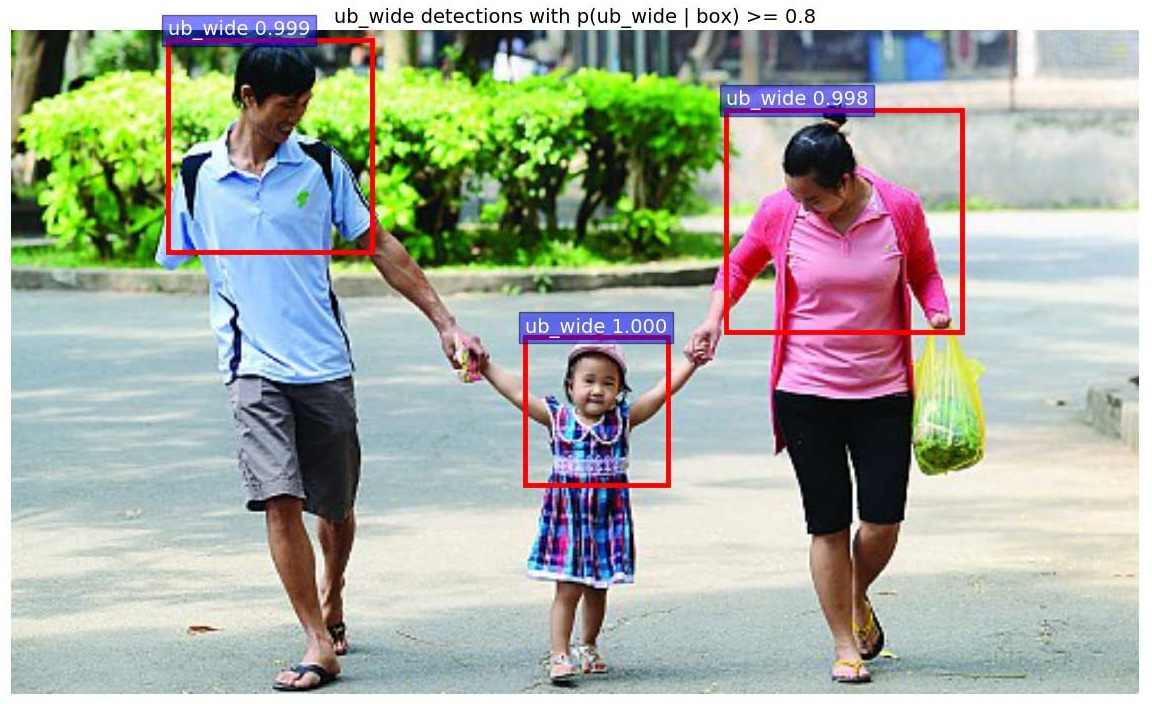
\includegraphics[width=\textwidth]{img5}
		\caption{}
		\label{fig:res5}
	\end{subfigure}
	~
	\begin{subfigure}[b]{0.3\textwidth}
		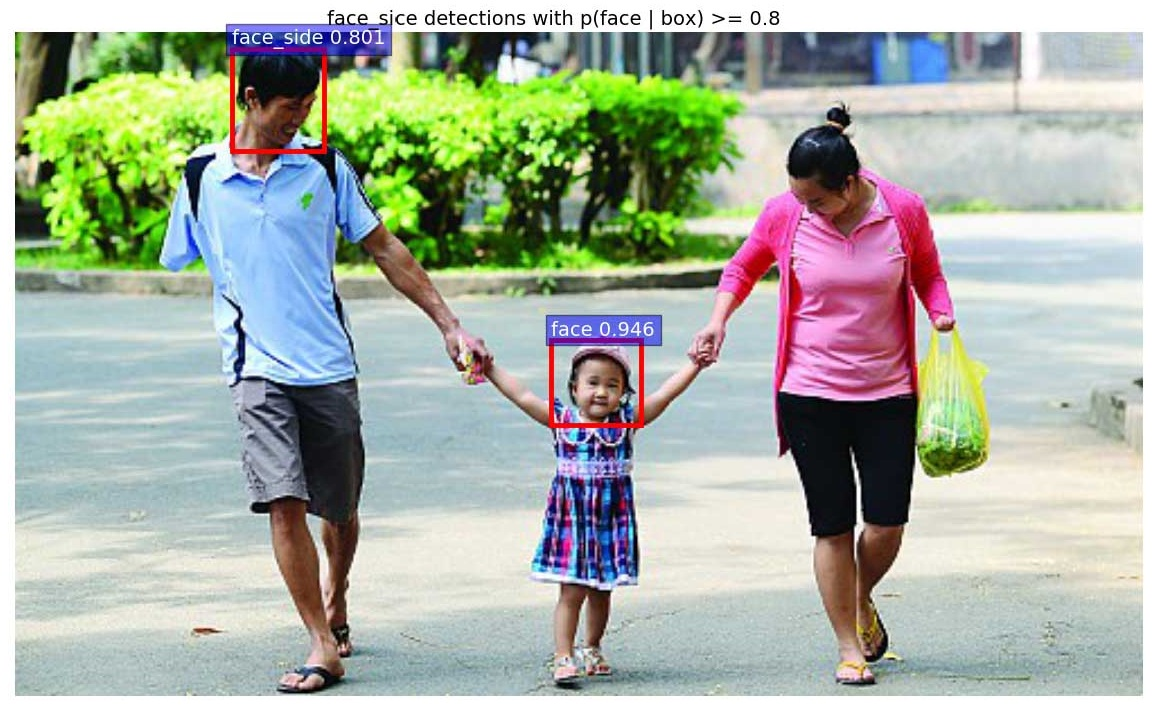
\includegraphics[width=\textwidth]{img6}
		\caption{}
		\label{fig:res6}
	\end{subfigure}
	\caption{Result pictures}\label{fig:animals}
\end{figure*}

And here we see in figure \ref{fig:res1}, most men's upper bodies are detected, except for 2 men on the left and 1 man on the right. This is because these upper bodies are not regular and the angles of their body are not included in the training set. 

In this case, R = 4/9 ( \(<50\) \%), 4 upper bodies are detected among 9 upper bodies.
this is still an encouraging result considering the complexity of this test case.


In figure \ref{fig:res2}, 5/6 upper bodies are detected despite some bodies are obscured and the image's quality is quite low. The undetected upper body is obscured and the color of the T-shirts also make it harder to detect in this test.

%\begin{table*}[H]
%\begin{tabular}{c c c}
%	%\hline
%	\addheight{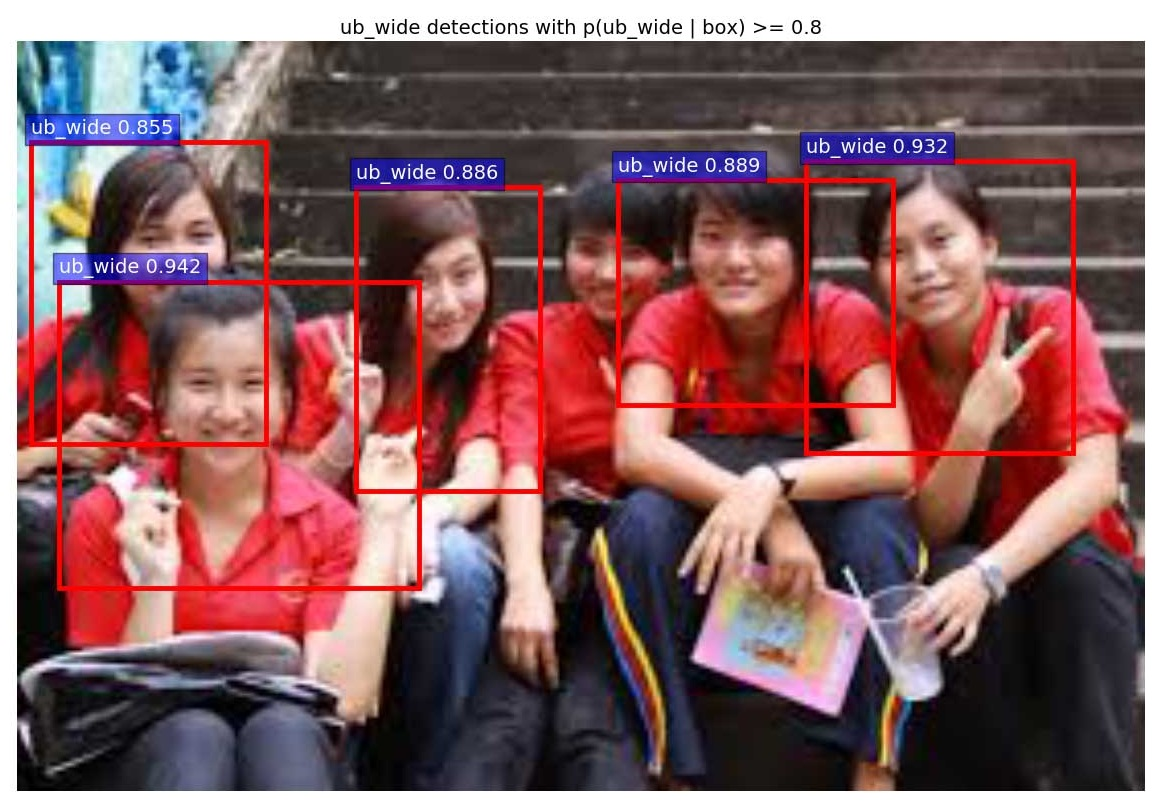
\includegraphics[width=60mm]{img2}} \label{fig:res2} &
%	\addheight{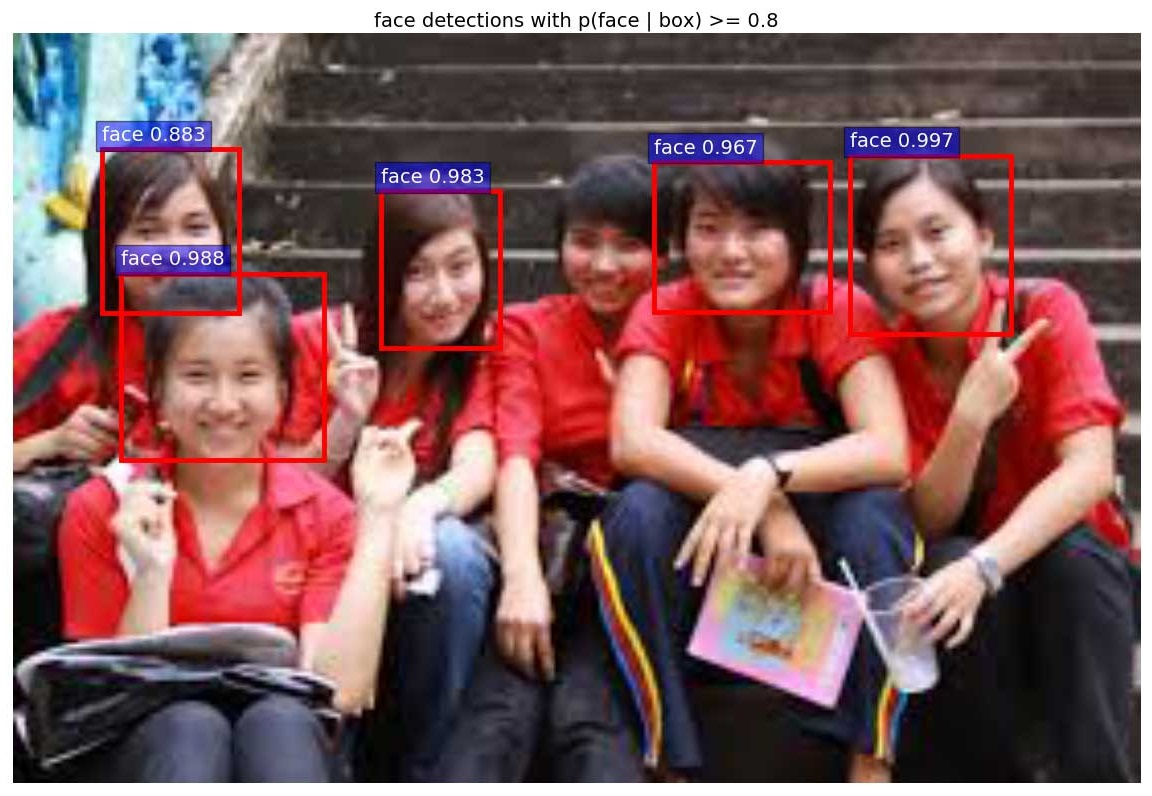
\includegraphics[width=60mm]{img3}} \label{fig:res3} &
%	\addheight{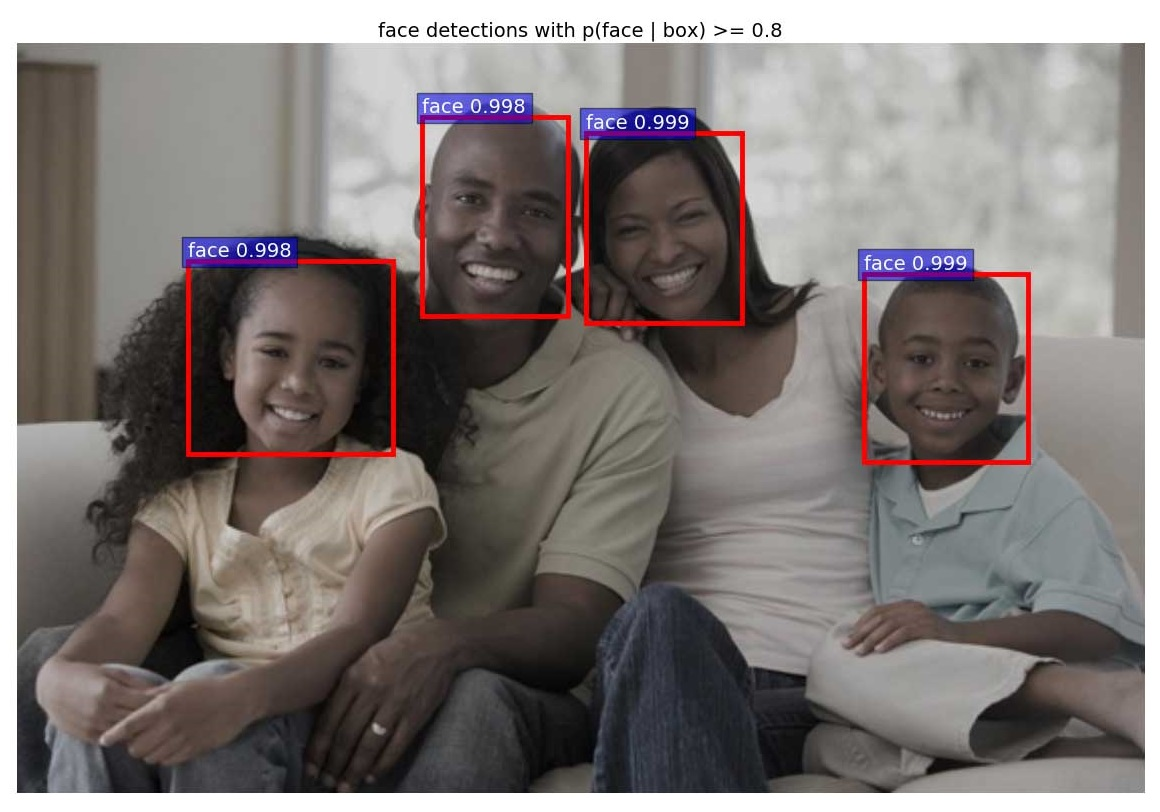
\includegraphics[width=60mm]{img4}} \label{fig:res4}	
%	\\
%	\small Result image 2 & Result image 3 &  Result image 4 \\
%	%\hline
%	\addheight{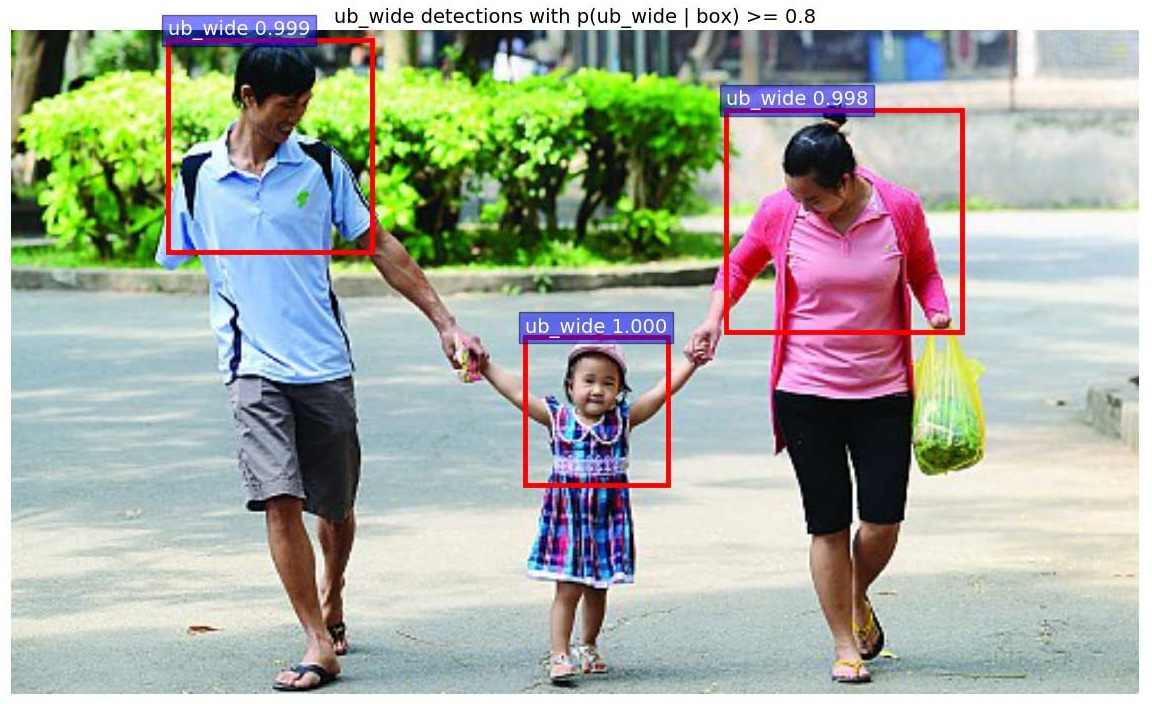
\includegraphics[width=60mm]{img5}} \label{fig:res5} &
%	\addheight{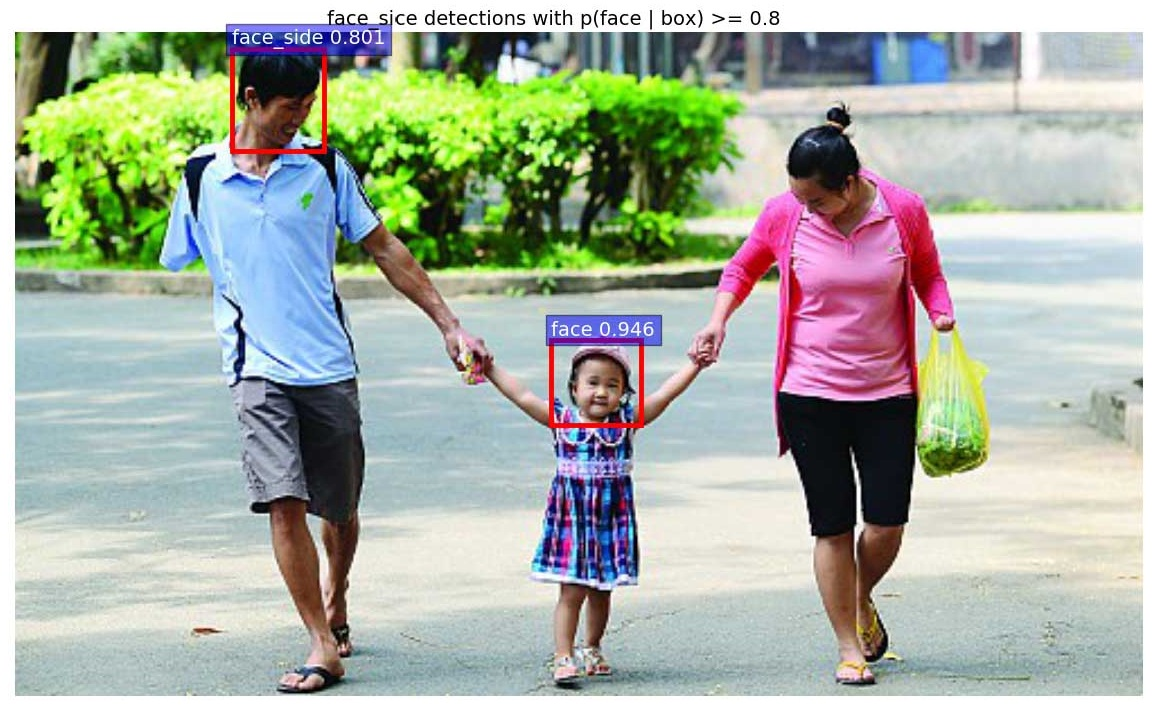
\includegraphics[width=60mm]{img6}} \label{fig:res6} &
%	\\
%	\small Result image 5 &  Result image 6 & \\
%	
%\end{tabular}
%\end{table*} 

In this test, the detector also found 5 faces, which are presented in \ref{fig:res3}. The undetected upper body's face is also undetected. This can be traced down to the limitation of the training stage, which only uses 98 images.

Still, this result is quit good, which gives R = 5/6 (about 83 \%)

In figure \ref{fig:res4}, all the upper bodies (and all faces) are detected with high certanties (\(> 0.95\)). This proves that in common cases, the detector can work well and give trusted result.
In this case, R = 1.

In figure \ref{fig:res5}, all upper bodies are detected correctly, which gives R = 1.

Only 2 out of 3 faces are detected. The last one is mostly obscured and too hard for the detector. \\
The average value of R = \(4/9 + 5/6 + 5/6 + 1 + 1) / 5 = 0.82\) \\

\section{Conclusion}

%The conclusion goes here.
Human detection is
%R-CNN is a powerful tools to address human detection problem. Howe
%\section{Future work}


% conference papers do not normally have an appendix


% use section* for acknowledgment
%\section*{Acknowledgment}

\pagebreak
\section*{}
\pagebreak






% trigger a \newpage just before the given reference
% number - used to balance the columns on the last page
% adjust value as needed - may need to be readjusted if
% the document is modified later
%\IEEEtriggeratref{8}
% The "triggered" command can be changed if desired:
%\IEEEtriggercmd{\enlargethispage{-5in}}

% references section

% can use a bibliography generated by BibTeX as a .bbl file
% BibTeX documentation can be easily obtained at:
% http://mirror.ctan.org/biblio/bibtex/contrib/doc/
% The IEEEtran BibTeX style support page is at:
% http://www.michaelshell.org/tex/ieeetran/bibtex/
%\bibliographystyle{IEEEtran}
% argument is your BibTeX string definitions and bibliography database(s)
%\bibliography{IEEEabrv,../bib/paper}
%
% <OR> manually copy in the resultant .bbl file
% set second argument of \begin to the number of references
% (used to reserve space for the reference number labels box)

\begin{thebibliography}{1}

\bibitem{wavelet}
M. M. Deshpande, J. G. Rana, and M. M. Pawar. \emph{"Human detection based on discrete Wavelet transform"}. Sustainable Energy and Intelligent Systems. IET Chennai International Conference. 3rd 2012.
\bibitem{hog}
N. Dalal and  B. Triggs. \emph{"Histograms of Oriented Gradients for Human Detection"}. Sustainable Energy and Intelligent Systems, IET Chennai International Conference, 3rd 2012.
\bibitem{rcnn}
Ross Girshick, Jeff Donahue, Trevor Darrell, and Jitendra Malik. \emph{"Region-based Convolutional Networks for Accurate Object Detection and Segmentation"}. IEEE Transactions on Pattern Analysis and Machine Intelligence, Volume 38.
\bibitem{slidingwin1} 
H. A. Rowley, S. Baluja, and T. Kanade. \emph{"Neural network-based face detection"}. TPAMI, 1998.
\bibitem{slidingwin2}
R. Vaillant, C. Monrocq, and Y. LeCun. \emph{"Original approach for the localisation of objects in images"}. IEE Proc on Vision, Image, and
Signal Processing, 1994.
\bibitem{slidingwin3}
Kevin Murphy, Antonio Torralba, Daniel Eaton, and William Freeman. \emph{"Object detection and localization using local and global features"}. Volume 4170 of the series Lecture Notes in Computer Science pp 382-400.
\bibitem{slidingwin4}
Anuj Mohan, Constantine Papageorgiou, and Tomaso Poggio. \emph{"Example-based object detection in images by components"}. IEEE Transactions on Pattern Analysis and Machine Intelligence, 23(4):349–361, 2001.
\bibitem{localinterestpoint1}
G. Bouchard and B. Triggs. \emph{"A hierarchical part-based model for visual object categorization"}. In CVPR, 2005.
\bibitem{slidingwin5}
Shaoqing Ren, Kaiming He, Ross Girshick, and Jian Sun. \emph{Faster R-CNN: Towards Real-Time Object	Detection with Region Proposal Networks}. Neural Information Processing Systems 2015.
\end{thebibliography}


% that's all folks
\end{document}


